\documentclass[a4paper,12pt]{article}

%%% Работа с русским языком
\usepackage{cmap}					% поиск в PDF
\usepackage{mathtext} 				% русские буквы в формулах
\usepackage[T2A]{fontenc}			% кодировка
\usepackage[utf8]{inputenc}			% кодировка исходного текста
\usepackage[english,russian]{babel}	% локализация и переносы
\usepackage{xcolor}
\usepackage{hyperref}
 % Цвета для гиперссылок
\definecolor{linkcolor}{HTML}{799B03} % цвет ссылок
\definecolor{urlcolor}{HTML}{799B03} % цвет гиперссылок

\hypersetup{pdfstartview=FitH,  linkcolor=linkcolor,urlcolor=urlcolor, colorlinks=true}

%%% Дополнительная работа с математикой
\usepackage{amsfonts,amssymb,amsthm,mathtools} % AMS
\usepackage{amsmath}
\usepackage{icomma} % "Умная" запятая: $0,2$ --- число, $0, 2$ --- перечисление

%% Номера формул
%\mathtoolsset{showonlyrefs=true} % Показывать номера только у тех формул, на которые есть \eqref{} в тексте.

%% Шрифты
\usepackage{euscript}	 % Шрифт Евклид
\usepackage{mathrsfs} % Красивый матшрифт

%% Свои команды
\DeclareMathOperator{\sgn}{\mathop{sgn}}

%% Перенос знаков в формулах (по Львовскому)
\newcommand*{\hm}[1]{#1\nobreak\discretionary{}
{\hbox{$\mathsurround=0pt #1$}}{}}
% графика
\usepackage{graphicx}
\graphicspath{{pictures/}}
\DeclareGraphicsExtensions{.pdf,.png,.jpg}
\author{Бурмашев Григорий, БПМИ-208}
\title{}
\date{\today}
\begin{document}
\maketitle
 \section*{Номер 11 [листок 5]}
Представим синус через тангенсы и по свойствам мат.ожидания получаем:
\[
\mathbb{E} \left(
\sin (2X) | \tg X 
\right) = \mathbb{E} \left(
\frac{2 \tg X}{1 + \tg^2 X} \Bigg| \tg X 
\right)  = \frac{2 \tg X}{1 + \tg^2 X} 
\]
\begin{center}
\textbf{Ответ: } 
\[
\frac{2 \tg X}{1 + \tg^2 X} 
\]
\end{center}
 \section*{Номер 12 [листок 5]}
\begin{center}
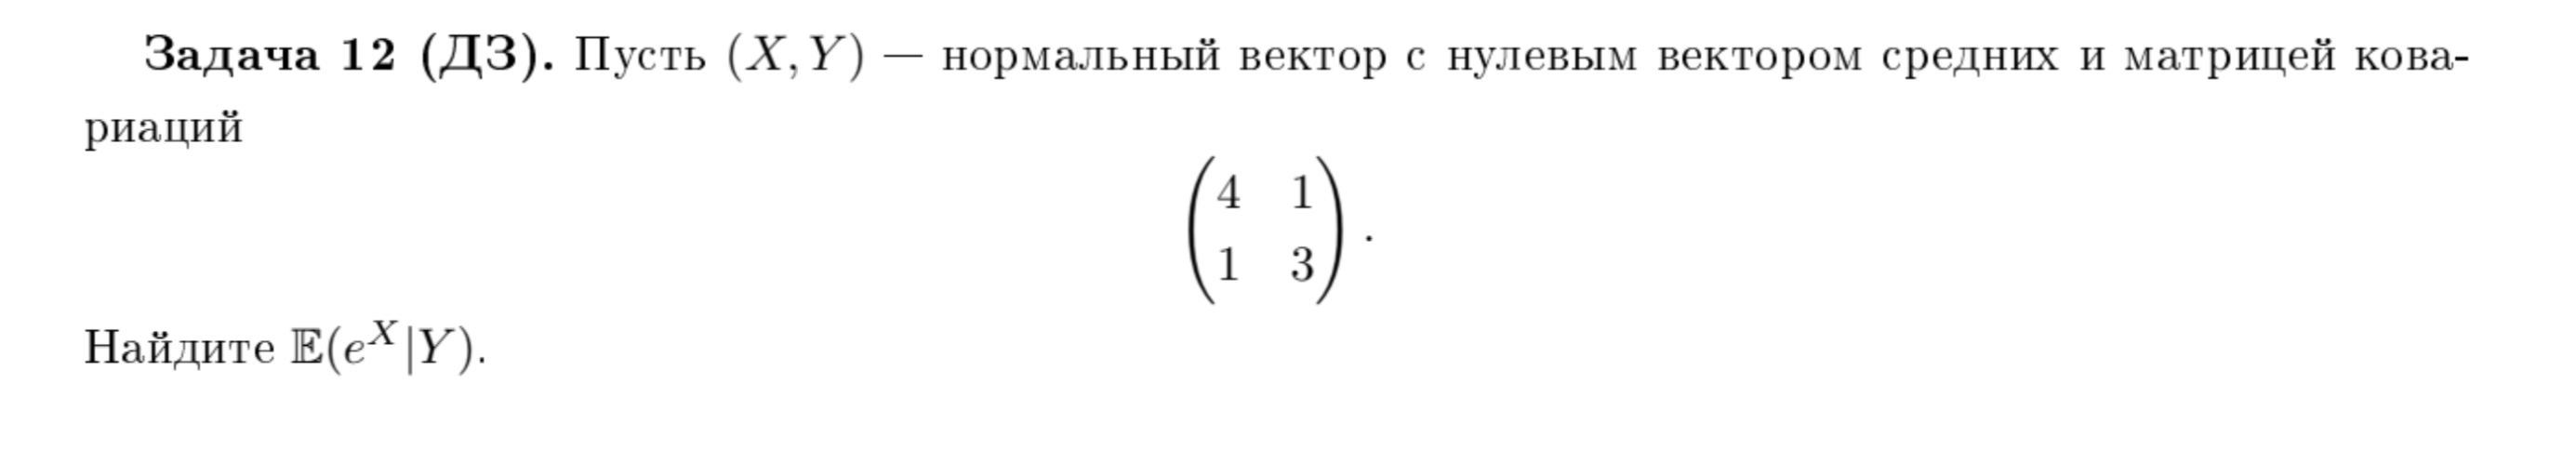
\includegraphics[scale=0.3]{1.png}
\end{center}
Хотим найти:
\[
\varrho_{X | Y} (x, y) = \frac{\varrho_{X, Y} (x, y)}{\varrho_Y(y)}
\]
Поработаем сначала с матрицей ковариаций, назовем её $R$:
\[
R = \begin{pmatrix}
4 & 1 \\ 1 & 3 
\end{pmatrix}
\]
Тогда:
\[
\det R = 11
\]
\[
R^{-1} = \left(\begin{matrix}
\frac{3}{11} & -\frac{1}{11} \\
-\frac{1}{11} & \frac{4}{11}
\end{matrix}\right)
\]
Ищем вспомогательные плотности (все данные знаем из матрицы ковариаций в условии):
\[
\varrho_Y(y) = \frac{1}{\sqrt{2\pi} \cdot \sqrt{3}} \cdot e^{-\frac12 \cdot \frac{1}{3} \cdot y^2}
\]
\[
\varrho_{X, Y} (x, y) = \frac{1}{2\pi \cdot \sqrt{11} } \cdot e^{-\frac{1}{2} \left(
\frac{3}{11} x^2 - \frac{2}{11}xy + \frac{4}{11y^2}
\right)}
\]
А значит:
\[
\varrho_{X | Y} (x, y)  = \frac{\frac{1}{2\pi \cdot \sqrt{11} } \cdot e^{-\frac{1}{2} \left(
\frac{3}{11} x^2 - \frac{2}{11}xy + \frac{4}{11}y^2
\right)}}{\frac{1}{\sqrt{2\pi} \cdot \sqrt{3}} \cdot e^{-\frac12 \cdot \frac{1}{3} \cdot y^2}} = \sqrt{\frac{3}{22}\pi } \cdot e^{-\frac{1}{2} \left(
\frac{3}{11} x^2 - \frac{2}{11}xy + \frac{1}{33}y^2 
\right)}
\]
Отсюда получаем мат.ожидание:
\[
\mathbb{E} (e^X | Y) = \int\limits_{-\infty}^{+\infty} e^x \cdot \sqrt{\frac{3}{22}\pi } \cdot e^{-\frac{1}{2} \left(
\frac{3}{11} x^2 - \frac{2}{11}xy + \frac{1}{33}y^2 
\right)} dx 
\]
\begin{center}
\textbf{Ответ: } 
\[
\mathbb{E} (e^X | Y) = \int\limits_{-\infty}^{+\infty} \left[ 
 e^x \cdot \sqrt{\frac{3}{22}\pi } \cdot e^{-\frac{1}{2} \left(
\frac{3}{11} x^2 - \frac{2}{11}xy + \frac{1}{33}y^2 
\right)} 
\right] 
dx 
\]
\end{center}
 \section*{Номер 2 [листок 5+]}
\begin{center}
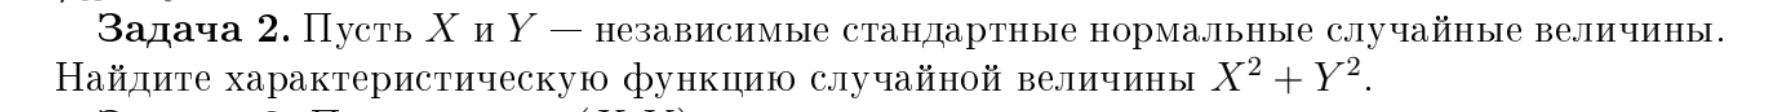
\includegraphics[scale=0.4]{2.png}
\end{center}
\[
\varphi_{X^2 + Y^2} = \mathbb{E} e^{it (X^2 + Y^2)} = \iint\limits_{R^2}  e^{it (X^2 + Y^2)} \cdot \varrho_{X, Y}(x, y) dx dy = \frac{1}{2\pi} \iint\limits_{R^2}  e^{it (x^2 + y^2)} \cdot e^{- \frac{x^2 + y^2}{2}} dx dy  = (\times)
\]
Делаем полярную замену:
\[
 (\times) = \frac{1}{2\pi} \int\limits_{0}^{2\pi} d \varphi  \int\limits_0^{+\infty} e^{itr^2} \cdot e^{-\frac{r^2}{2}} r dr = \int\limits_0^{+\infty} e^{r^2 \cdot \left(it - \frac12\right)} \cdot \frac12 dr^2 = \frac12 \cdot \frac{e^{(it - \frac12)r^2}}{it - \frac12 } \Bigg|_0^{+ \infty} = \frac{1}{1 - 2it}
\]
\begin{center}
\textbf{Ответ: } 
\[
\frac{1}{1 - 2it}
\]
\end{center}
\end{document}
